
\newcommand{\param}[2]{\textit{#1}\,--\,#2\,--\,}
\newcommand{\paramnott}[2]{#1\,--\,#2\,--\,}

\chapter{Praktická část}
Praktická část práce se skládá ze~dvou častí. První část je implementace samotného protokolu L2RS (Lattice-based one-time Link-able Ring Signature) a~druhá část je ukázková aplikace, která využívá implementaci protokolu. Sekce níže popisují jednotlivé části práce.

\section{Protokol L2RS}
Protokol L2RS je implementovaný v jazyce Python a jako jedinou knihovnu využívá \texttt{numpy}. Parametry pro protokol byly zvolené následovně:

\begin{itemize}
  \item \param{q}{12289}modulus pro koeficienty v polynomech,
  \item \param{n}{512}počet koeficientů v polynomech,
  \item \param{m}{6}počet polynomů v jednom vektoru,
  \item \paramnott{$\sigma$}{283754}standardní Gaussova odchylka,
  \item \paramnott{$\gamma$}{13.6}hustota privátního klíče.
\end{itemize}

Tyto parametry byly zvolené, aby splňovaly bezpečnostní úroveň \texttt{III} protokolu \cite{Torres2018}. Vytváření podpisu trvá průměrně 43\,ms a ověření průměrně 38\,ms při výše opomenutých parametrech. Rychlost podpisu a ověření je samozřejmé závislá na parametrech stroje, na kterém byly testované. Tyto časy byly měřené na procesoru AMD Ryzen 3600 s frekvencí jádra 3.6\,GHz.

V tabulce \ref{sizes} je možné vidět velkosti jednotlivých konstrukcí jako veřejný nebo~privátní klíč. Velikosti podpisu jsou lineárně závislé na počtu uživatelů, kteří se zúčastňují podpisu. Velikost podpisu se dá jednoduše vypočítat podle rovnice:
\begin{equation}
  S=1792+w*m*896
\end{equation}
kde $w$ označuje počet uživatelů, kteří veřejně poskytují veřejný klíč na vytvoření podpisu, a $m$ označuje počet polynomů v jednom vektoru.


\begin{table}[htbp]
  \centering
  \caption{Velikosti konstrukcí podpisů}
  \begin{tabular}{|l|c|r|}
    \hline
    Typ              & Počet uživatelů & Velikost (B) \\
    \hline
    Veřejný klíč     & -               & 896         \\
    Privátní klíč    & -               & 4 480        \\
    Veřejný parametr & -               & 8 960        \\
    Podpis           & 1               & 7 168        \\
    Podpis           & 2               & 12 544       \\
    Podpis           & 5               & 28 672       \\
    \hline
  \end{tabular}
  \label{sizes}
\end{table}


\section{Ukázková aplikace}
Součást práce je taktéž ukázková aplikace, která vyváří komunikaci mezi uživateli, kteří jsou schopní ověřovat vytvořené podpisy. Aplikace se skládá ze~tří částí: \textbf{proxy server}, \textbf{podpisovatel} a \textbf{ověřovatel}. Jak je možné vidět na obrázku \ref{network_diagram}, proxy server přeposílá generovaný podpis všem připojeným ověřovatelům. Také se~stará o~generovaní veřejných parametrů, které posílá na vyžádaní uživatelům. Uživatel může být ověřovatel nebo podpisovatel. 

Podpis se generuje jenom jedním podpisovatelem s využitím soukromého klíče, veřejných parametrů a veřejných klíčů všech účastníku. Veřejné klíče jsou zasílané uživateli proxy serveru, když se poprvé připojí a vygenerují si soukromý a veřejný klíč. Proxy server stejně jako veřejné parametry poskytuje i posbírané veřejné klíče na vyžádání. Když podpisovatel zašle vygenerovaný podpis na zprávu, která byla zadaná, je přeposlána všem uživatelům, aby ji mohli ověřit pomocí veřejných parametrů, veřejných klíčů všech účastníku a originální zprávy.

\begin{figure}[htbp]
  \centering
  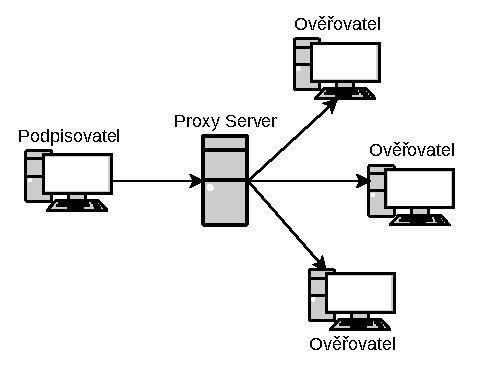
\includegraphics[width=0.65\textwidth]{img/network_diagram.pdf}
  \caption{Síťová komunikace}
  \label{network_diagram}
\end{figure}

Stanice si mezi sebou zprávy vyměňují pomocí protokolu TCP s~jednoduchou aplikační hlavičkou, jehož formát je možné vidět na obrázku \ref{header}. Políčko \texttt{typ} zprávy označuje co je obsahem zprávy. Typy zpráv jsou následovné:
\begin{itemize}
  \item \texttt{NEED\_PUB\_PARAMS} -- uživatel požaduje veřejné parametry,
  \item \texttt{PUB\_PARAMS} -- server posílá veřejné parametry,
  \item \texttt{MY\_PUB\_KEY} -- uživatel zasílá svůj veřejný klíč,
  \item \texttt{NEED\_PUB\_KEYS} -- uživatel požaduje veřejné klíče všech uživatelů,
  \item \texttt{PUB\_KEYS} -- server posílá veřejné klíče všech uživatelů,
  \item \texttt{SIGNATURE} -- uživatel nebo server zasílá podpis na ověření.
\end{itemize}

\begin{figure}[htbp]
  \centering
  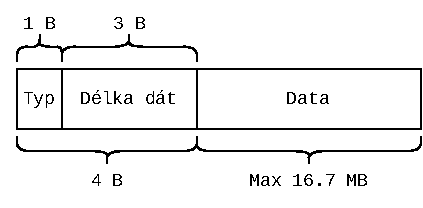
\includegraphics[width=0.7\textwidth]{img/header.pdf}
  \caption{Aplikační hlavička}
  \label{header}
\end{figure}

\subsection{Návod na použití}
Program používá přepínače na jeho ovládaní. Spuštění je možné ve Windows powershellu, WSL (Windows Subsystem for Linux) nebo libovolné Linux distribuci. Program byl testovaný na verzi \texttt{Python 3.10.7}. Návod na spuštění je následovný. Jako první je potřeba nainstalovat potřebné balíčky pomocí souboru \texttt{requirements.txt}, který se nachází v odevzdaném kódu:
\begin{itemize}
  \item \texttt{pip install -r requirements.txt}
\end{itemize}
Spustit \textbf{pouze jeden} proxy server:
\begin{itemize}
  \item \texttt{./ring\_sig.py -sp}
\end{itemize}
Spustit \textbf{pouze jednoho} podpisovatele:
\begin{itemize}
  \item \texttt{./ring\_sig.py -c -s}
\end{itemize}
Spustit \textbf{libovolný počet} ověřovatelů:
\begin{itemize}
  \item \texttt{./ring\_sig.py -c -v}
\end{itemize}
Dále stačí jednom zadat text, který bude podepsaný a ověřený u každého ověřovatele. Jako předvolené nastavení používá program port \textbf{6000} pro komunikaci. Tento port je možné změnit pomocí přepínače \texttt{-p}.
\begin{itemize}
  \item \texttt{./ring\_sig.py -p [PORT]}
\end{itemize}
Všechny dostupné přepínače se dají zobrazit pomocí:
\begin{itemize}
  \item \texttt{./ring\_sig.py -h}
\end{itemize}
Dále je možné zobrazit jednotlivé parametry, které jsou použité pro protokol L2RS a~síťovou komunikaci:
\begin{itemize}
  \item \texttt{./ring\_sig.py -i}
\end{itemize}


